\documentclass[utf8]{gradu3}
% Jos työ on kandidaatintutkielma eikä pro gradu, käytä ylläolevan asemesta
%\documentclass[utf8,bachelor]{gradu3}
% Jos kirjoitat englanniksi, käytä ylläolevan asemesta
%\documentclass[utf8,english]{gradu3}
% tai
%\documentclass[utf8,bachelor,english]{gradu3}

\usepackage{graphicx} % kuvien mukaan ottamista varten

\usepackage{amsmath} % hyödyllinen jos tekstisi sisältää matikkaa,
                     % ei pakollinen

\usepackage{booktabs} % hyvä kauniiden taulukoiden tekemiseen

\usepackage[authordate,backend=biber,noibid]{biblatex-chicago} % biber / chicago-tyylin käyttö

\usepackage{graphicx} % kuvien lisääminen

% HUOM! Tämän tulee olla viimeinen \usepackage koko dokumentissa!
\usepackage[bookmarksopen,bookmarksnumbered,linktocpage]{hyperref}

\addbibresource{gradu_EK.bib} % Lähdetietokannan tiedostonimi

\begin{document}

\title{Vertaileva tutkimus koneoppimisen hyödyntämisestä videopelien reitinhaussa}
\translatedtitle{Comparative study of utilizing machine learning in video games' pathfinding}
\studyline{Tietotekniikka}
\tiivistelma{%
TODO: tiivistelmä suomeksi
}
\abstract{%
TODO: In english
}

\author{Emil Keränen}
\contactinformation{\texttt{emil.a.keranen@student.jyu.fi}}
% jos useita tekijöitä, anna useampi \author-komento
\supervisor{Tommi Kärkkäinen}
% jos useita ohjaajia, anna useampi \supervisor-komento
\avainsanat{koneoppiminen, videopeli, reitinhaku, syvä vahvistusoppiminen}
\keywords{machine learning, video game, pathfinding, deep reinforcement learning, Soft Actor Critic, Machine Learning Agents, Unity}

\maketitle

\bigskip

\mainmatter

\chapter{Johdanto}

- Tutkimuksen kohteena koneoppimisen tehostama reitinhaku videopeleissä
 ja sen vertaaminen heuristiseen A*-algoritmiin.

- Yleisesti reitinhaulla tarkoitetaan alku- ja loppupisteen välisen reitin selvittämistä. Useimmiten tarkoituksena
on löytää lyhin reitti väistellen samalla matkan varrella olevia esteitä.

- Reitinhakua tarvitaan videopelien lisäksi myös mm. robotiikassa. 

- Videopeleissä reitinhaku ilmenee pääasiassa tekoälyagenttien suorittamana toimintana, joten tässä tutkimuksessa keskitytään agentteihin.
Näitä agentteja kutsutaan myös ei-pelaaja-hahmoiksi (engl. non-player-character, NPC).

- Ei-pelaaja-hahmot ja itseasiassa videopelien reitinhaku vertautuvat hyvin robotiikkaan ja robottien reitinhakuun.

- Sekä robotiikassa että videopeleissä toiminta-alue voi muuttua hyvinkin paljon reaaliajassa, jolloin reitinhaun täytyy
sopeutua muutoksiin nopeasti. Käytetyt ratkaisut sen sijaan voivat vaihdella näiden kahden osa-alueen välillä: robotiikassa
tarkkuus ja turvallisuus nousevat tärkeimmiksi ominaisuuksiksi ja vastaavasti videopeleissä nopeus määrittää reitinhaun "hyvyyden".

- Reitinhaku on aina ollut vaativa ongelma videopeleissä, mutta nykyään reitinhaun ongelmallisuus voidaan
useimmissa tapauksissa sivuuttaa laatimalla heuristinen ratkaisu A*-algoritmin avulla.

- Koneoppiminen mahdollistaa aiemman kokemuksen hyödyntämisen myöhemmässä toiminnassa.
Agentteja voidaan kouluttaa harjoitteludatan avulla, jolloin ne oppivat toimimaan tuntemattomissa tilanteissa.
Koneoppimisen ansiosta reitinhaku-agentti voidaan opettaa toimimaan vaativissa ja
dynaamisissa pelialueissa, joissa muuttuvat esteet ja alueen labyrinttimäisyys
heikentävät A*-algoritmin toimintaa.

- Tutkimuksen ideana on käyttää Unity-pelimoottorille luotuja koneoppimisagentteja (engl. Unity Machine Learning Agents)
ja opettaa niitä erilaisten pelialueiden avulla. Opettamisen jälkeen agentteja testataan oikeilla
pelialueilla ja verrataan tuloksia A*-algoritmilla saatuihin tuloksiin.

- ML-agents perustuu PyTorch-kirjastoon ja mahdollistaa vahvistusoppimisen hyödyntämisen.

- Tensorboard-lisäosan avulla voidaan visualisoida palkkioiden keskiarvot ja opetuksen edistyminen opetuksen aikana.

- Pelialueiden on tarkoitus olla monimutkaisia ja dynaamisia, koska A*-algoritmi suoriutuu
yksinkertaisista reitinhakutehtävistä moitteettomasti.

\chapter{Reitinhaku videopeleissä}

Reitinhaulla tarkoitetaan yksinkertaisimmillaan reitin selvittämistä kahden pisteen välillä. Se on yksi videopelien tekoälyn ja myös robotiikan tunnetuimmista ja haastavimmista ongelmista, jota on tutkittu jo muutaman vuosikymmenen ajan \parencite{cui2011based,abd2015comprehensive}. Reitinhakua esiintyy monissa eri peligenreissä, kuten roolipeleissä ja reaaliaikaisissa strategiapeleissä, joissa ei-pelaaja-hahmoja (non-player-character, NPC) määrätään liikkumaan ennaltamäärättyyn tai pelaajan määräämään sijaintiin väistellen samalla vastaantulevia esteitä \parencite{cui2011based}.

\section{Pelialueen esitystavat}

Yleisin alueen esittämistapa on ruudukko (engl. grid), joka sisältää yksittäisiä ruutuja (engl. tile). Ruudut merkitään ennalta vapaiksi tai esteiksi. Vapaista ruuduista muodostetaan verkko, jolloin jokainen vapaa ruutu vastaa yhtä verkon solmuista. Vierekkäisiä solmuja yhdistävät linkit, joita pitkin reitinhaku tapahtuu. Solmujen vierekkäisyys voi tarkoittaa horisontaalista ja vertikaalista vierekkäisyyttä (neljä suuntaa) tai näiden lisäksi myös diagonaalista vierekkäisyyttä (kahdeksan suuntaa). \parencite{botea2013pathfinding,abd2015comprehensive}. Kuvio \ref{ruudukkokuva} havainnollistaa yksinkertaista ruudukkoaluetta, jossa liikkuminen tapahtuu neljään suuntaan.

\begin{figure}[h]
\centering
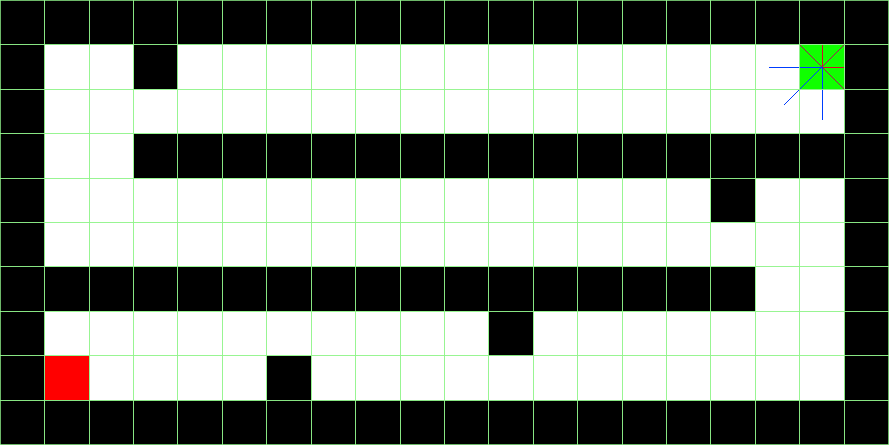
\includegraphics[width=15cm]{ruudukko_kuva.png}
\caption{Ruudukko, jossa mustat ruudut ovat esteitä ja valkoiset ruudut vapaita. Vihreä ruutu on aloitusruutu ja punainen ruutu on maaliruutu. Vihreästä ruudusta lähtevät säteet ovat mahdollisia etenemissuuntia.}
\label{ruudukkokuva}
\end{figure}

Vähemmän käytettyjä alueen esitystapoja ovat kolmiointi ja kuusikulmiointi (oikea termi kuusikulmioinnista?) \parencite{abd2015comprehensive}. Alueen kolmiointi ja siihen perustuvat TA*- ja TRA*-algoritmi ovat kuitenkin osoittautuneet moninkertaisesti nopeammiksi suurissa pelialueissa verrattuna A*-algoritmiin \parencite{demyen2006efficient}. Kuusikulmioihin perustuvat alueet ja reitinhakualgoritmit ovat myös tuottaneet lupaavia tuloksia muun muassa robotiikan tutkimuksessa \parencite{abd2015comprehensive}.

\section{Reitinhakualgoritmit}

Graafin lyhyimmän polun ongelmaa on tutkittu jo vuosikymmenten ajan. Vanhimmat ja tunnetuimmat algoritmit, Dijkstran algoritmi \parencite{dijkstra1959note} ja A*-algoritmi \parencite{hart1968formal}, esiteltiin jo 50- ja 60-luvuilla. A*-algoritmi on selvästi tunnetumpi videopelien ja robottien reitinhaussa nopeutensa ansiosta \parencite{cui2011based,abd2015comprehensive,botea2013pathfinding}. Tässä tutkimuksessa keskitytään tarkemmin A*-algoritmiin ja sen variaatioihin.

\subsection{A*-algoritmi}

A*-algoritmi on hyvin tunnettu paras-ensin -reitinhakualgoritmi (termi kuntoon?), joka hyödyntää heuristista arviointifunktiota lyhimmän reitin etsimiseen \parencite{cui2011based,duchovn2014path}.

Algoritmin toiminta tapahtuu seuraavasti: jokainen aloitussolmun vierekkäinen solmu arvioidaan kaavan \[f(n)=h(n)+g(n)\] mukaisesti, jossa \(n\) on solmu, \(h(n)\) on heuristinen etäisyys solmusta \(n\) maalisolmuun ja \(g(n)\) on todellinen etäisyys aloitussolmusta solmuun \(n\). Näistä solmuista matalimman \(f(n)\)-arvon solmu käsitellään seuraavaksi, jolloin kyseisen solmun vierekkäisten solmujen \(f(n)\)-arvot lasketaan. Tämä prosessi jatkuu, kunnes maalisolmu saavutetaan. Heuristiikan ollessa nolla A*-algoritmista tulee Dijkstran algoritmi.

A*-algoritmilla on kolme esitettyä ominaisuutta \parencite{hart1968formal}. A*-algoritmi löytää reitin, jos sellainen on olemassa. Reitti on optimaalinen, jos heuristiikka on luvallinen(admissible?) eli arvioitu etäisyys on lyhyempi tai yhtä suuri kuin todellinen etäisyys. Lopuksi mikään muu algoritmi samalla heuristiikalla ei käy läpi vähemmän solmuja kuin A*-algoritmi eli A* käyttää heuristiikkaa tehokkaimmalla mahdollisella tavalla. \parencite{hart1968formal,cui2011based}. Luvallisia heuristiikkoja ovat solmujen vierekkäisyydestä riippuen Euklidinen etäisyys, Manhattan-etäisyys, Chebyshev-etäisyys ja Octile-etäisyys \parencite{duchovn2014path,botea2013pathfinding}. Manhattan-etäisyyttä käytetään pääasiassa neljän suunnan ja Octile- sekä Chebyshev-etäisyyttä kahdeksan suunnan vierekkäisyyksissä \parencite{botea2013pathfinding}. Euklidista etäisyyttä voidaan käyttää tilanteessa, jossa 

\subsection{A*-algoritmin variaatiot}

A*-algoritmin heikkous on huono skaalautuvuus suurien alueiden reitinhakuun. Esimerkiksi kaksiulotteisessa ja esteettömässä 1000x1000 ruudukkoalueessa solmuja on miljoona, jolloin A*-algoritmin muistinkäyttö ja nopeus koituvat ongelmaksi. \parencite{cui2011based,duchovn2014path} Tämä ongelma esiintyy videopelien lisäksi etenkin robotiikassa, jonka seurauksena A*-algoritmi on inspiroinut tutkijoita monien eri variaatioiden kehittämiseen, kuten Theta*-, Phi*- ja HPA*-algoritmit \parencite{duchovn2014path}.

\section{Reitinhaun ongelmat}

Reitinhaun on oltava videopeleissä nopeaa ja laskennallisesti tehokasta. Lisäksi reittien on näytettävä realistiselta pelaajalle. Yhden agentin staattisen ruudukkoalueen reitinhakuongelma on ratkaistavissa nopeasti ja tehokkaasti heuristisella A*-algoritmilla, mutta nykyään videopeleissä reitinhakuongelmat ovat monimutkaisempia. Reitinhakuongelmat pitävät sisällään esimerkiksi useamman agentin samanaikaista reitinhakua ja reaaliajassa muuttuvien alueiden reitinhakua. Nykytutkimus keskittyykin pääasiassa monimutkaisiin reitinhakuongelmiin.

Useamman agentin samanaikaisessa reitinhaussa alueella on useampi kuin yksi agentti ja jokaisella niistä on oma aloitus- ja lopetuspisteensä. Jos jokaisen agentin reitinhakuun sovelletaan A*-algoritmia suurella 1000x1000 pelialueella, muistiin joudutaan tallentamaan miljoona solmua yhtä agenttia kohden. Muistinkäytön lisäksi jokaisen agentin täytyy tarvittaessa väistää toisia agentteja ja mahdollisesti muita esteitä. A*-algoritmi osoittautuu riittämättömäksi ongelman ratkaisuun.

\chapter{Koneoppiminen}

- Keskeiset koneoppimiseen liittyvät kysymykset: Kuinka saada tietokone oppimaan kokemuksen kautta? Voidaanko oppimista jäljitellä?

- Koneoppimisella pyritään luomaan tietokoneelle mahdollisuus oppia aiemmasta kokemuksesta.

- Koneoppimisella ei ole selkeää omaa alaansa, vaan se sijoittuu tietotekniikan ja tilastotieteen välille. Se on kuitenkin selkeästi tekoälyn ja dataopin ytimessä.

- Suurista datajoukoista oppiminen ja erilaisten ennusteiden tekeminen ja päätöksenteko vaatii tilastotieteellisiä menetelmiä.

- Koneoppiminen on noussut vuosikymmenten saatossa tärkeäksi teknologiaksi sekä tutkimuksen että kaupallisten tuotteiden parissa.

- Laskentatehon kasvu, uudet oppimisalgoritmit ja suuret datamäärät (big data) ovat sekä tuoneet tarpeen koneoppimisratkaisuille sekä mahdollistaneet koneoppimisen laajan hyödyntämisen.

- Koneoppiminen ja syöte-tuloste -esimerkkien avulla opettaminen voi osoittautua paljon helpommaksi verrattuna manuaaliseen opettamiseen, jossa jokaiselle syötteelle asetetaan haluttu tulos. (tämä lause uusiksi)

- Monet tieteenalat ovat alkaneet hyödyntämään koneoppimista eri sovellusten parissa.

- Tunnettuja esimerkkejä ovat konenäkö, puheentunnistus ja robotiikka. Konenäköä hyödynnetään etenkin terveydenhoidon alalla anomalioiden tunnistamiseen kuvissa. Mainonnassa koneoppimista käytetään personoitujen suositusten luomiseen ja markkinoinnissa erilaisissa ennusteissa.

- Oppimisongelman voi selittää lyhyesti jonkin mitattavan asian tai suorituskyvyn kohentamisena kokemuksen kautta. Luokitteluongelmat (on/ei) ovat yleisiä oppimiseen liittyviä ongelmia.

-Ohjattu oppiminen on koneoppimisen osa-alue, jossa oppiminen tapahtuu luokitellun aineiston perusteella. Ohjattu oppiminen havainnollistaa lineaariapproksimaatiota ja siihen liittyviä ongelmia. Opetusaineisto tuodaan \((x,y)\) pareina, jossa \(x\) on syöte, esimerkiksi kuva, ja \(y\) on tulos, esimerkiksi lintu. Oppijan tavoitteena on tuottaa ennuste \(y\) syötteen \(x\) perusteella.

- Ohjaamaton oppiminen mahdollistaa koneoppimisen ilman ihmisen apua tai väliintuloa. Ohjaamattomassa oppimisessa pyritään tunnistamaan datan rakenteet ja mallit ilman datan valmista luokittelua.

- Vahvistusoppiminen sijoittuu ohjatun ja ohjaamattoman oppimisen väliin. Harjoitusdata on vain osittain luokiteltua, ja suurin osa oppimisesta tapahtuu kokeilemalla. Tietylle syötteelle \(x\) ei siis anneta valmiiksi oikeaa tulosta \(y\), vaan agentti saa jokaisesta toiminnasta positiivisen tai negatiivisen palautteen tai palkkion. Agentin tarkoituksena on maksimoida palkkioiden summa tehtävää suorittaessa. Vahvistusoppimisesta selitetään luvussa \ref{sec:vahvistusoppiminen} lisää.

LÄHDE: (\parencite{jordan2015machine})

\section{Neuroverkot ja syväoppiminen}

- 

\section{Vahvistusoppiminen ja syvä vahvistusoppiminen}
\label{sec:vahvistusoppiminen}

Vahvistusoppiminen on koneoppimisen osa-alue, jonka tavoitteena on opettaa ja ohjata agentin käyttäytymistä yrityksen ja erehdyksen kautta (Reinforcement Learning: A Survey, Reinforcement learning: An introduction?). Agentti on jatkuvassa vuorovaikutuksessa ympäristönsä kanssa ja tarkkailee samalla toimintojensa vaikutusta ympäristössä. Agentin oppimisprosessia ja käyttäytymistä ohjataan palkkioilla (a brief survey of deep reinforcement learning).

Vahvistusoppimisen malli voidaan kuvata tilojen \(S\), toimintojen \(A\) ja palkkiosignaalien \(r\) avulla. Jokaisella aika-askeleella \(t\) agentti suorittaa toiminnan \(a\), jolloin ympäristön tila \(s\) muuttuu ja muutos viestitään agentille palkkiosignaalin \(r\) kautta. Palkkiosignaalin lisäksi ympäristö viestii agentille tilamuutoksesta, jolloin agentti saa tiedon uudesta tilasta \(s+1\). Palkkion ja uuden tilan perusteella agentti valitsee jälleen seuraavan toimintonsa. Agentin lopullisena tavoitteena on saavuttaa paras mahdollinen käytäntö (engl. policy), joka maksimoi saadun palkkion määrän (a brief survey of drl).

TODO: rise of drl eteenpäin, actor-critic menetelmästä asiaa?

\section{Soft-Actor Critic -algoritmi}

Soft Actor-Critic on Haarnojan ym. kehittämä algoritmi, joka perustuu syvään vahvistusoppimiseen \parencite{haarnoja2018soft}. 

\chapter{Unity}

Unity on Unity Technologiesin kehittämä pelinkehitysalusta, joka sisältää oman renderöinti- ja fysiikkamoottorin sekä Unity Editor -nimisen graafisen käyttöliittymän \parencite{juliani2018unity}. Unityllä on mahdollista kehittää perinteisten 3D- ja 2D-pelien lisäksi myös esimerkiksi VR-pelejä tietokoneille, mobiililaitteille ja pelikonsoleille. Unitystä onkin vuosien mittaan tullut yksi tunnetuimmista pelinkehitysalustoista, jonka parissa työskentelee kuukausittain jopa 1.5 miljoonaa aktiivista käyttäjää \parencite{unityweb}.

Viime vuosina Unityä on käytetty simulointialustana tekoälytutkimuksen parissa. Unity mahdollistaa lähes mielivaltaisten tilanteiden ja ympäristöjen simuloinnin 2D ruudukkokartoista monimutkaisiin pulmanratkaisutehtäviin, joka on sen suurimpia vahvuuksia simulointialustana. Kehitystyö ja prototypointi ovat Unityllä myös erityisen nopeaa. \parencite{juliani2018unity}.

\section{Unityn hierarkia}

Tässä luvussa käsitellään Unityn hierarkiaa. Aliluvuissa käydään läpi hierarkian osat ylimmästä lähtien.

\subsection{Unity-projekti}

Unityn hierarkian ylin osa on projekti, jonka luomisesta kehitystyö aina alkaa. Unityssä on mahdollista luoda projekti valmiista pohjista, joita ovat esimerkiksi 2D-, 3D- ja VR-pohjat. Pohjien avulla projekteihin saa lisättyä suoraan suositeltavat, parhaita käytäntöjä mukailevat asetukset.

Unity-projekteja voidaan hallinnoida ja avata erillisellä Unity Hub -sovelluksella. Unity Hub kertoo muun muassa mitä Unityn versiota projekti tukee. Projekteja voi tarvittaessa siirtää (engl. migrate) toimimaan uusimmilla Unityn versioilla, mutta siirto voi aiheuttaa toiminnallisuuksien muutoksia tai virheitä projektissa.

\subsection{Näkymät}

Projektista seuraavana hierarkiassa ovat näkymät (engl. scene). Näkymät toimivat työskentelyalustoina projektissa. Projekti sisältää aina yhden tai useamman näkymän, koska ilman niitä mitään ei pysty luomaan. Tavallisesti yksittäinen näkymä kuvaa aina yhtä kenttää, tasoa tai aluetta pelissä, ja siirryttäessä toiselle alueelle Unity pystyy lataamaan ajon aikana uuden skenen. Näkymän lataaminen voi tosin viedä aikaa, joten lataus peitetään useimmiten latausruuduilla, jotka voivat myös olla omia, yksinkertaisia näkymiä. Yksinkertaisimmillaan peli voi kuitenkin sisältää vain yhden näkymän, joka muokkautuu ja jota muokataan ajon aikana.

Projektin luonnin jälkeen Unity lisää siihen automaattisesti aloitusnäkymän, joka sisältää kamera- ja valonlähde-peliobjektin. Tätä näkymää voi lähteä muokkaamaan lisäämällä siihen erilaisia peliobjekteja, esimerkiksi maata ja erilaisia geometrisia muotoja.

\subsection{Peliobjektit ja Prefabit}

Peliobjektit (engl. GameObject) ovat tärkein osa Unityn pelinkehitysprosessia, koska kaikki peliin luotavat objektit ovat taustaltaan peliobjekteja. Peliobjektit eivät itsessään tee mitään tai näytä miltään, vaan ne toimivat säiliöinä komponenteille. Peliobjekteja voidaan järjestellä vanhempi-lapsi -periaatteella. Lapsiobjektit liikkuvat vanhemman mukana, jolloin niitä ei tarvitse liikutella näkymässä erikseen. Kuvio \ref{peliobjektikuva} havainnollistaa esimerkkinäkymän peliobjekteja ja niiden vanhempi-lapsi -suhteita.

Prefabit ovat peliobjektien valmiita malleja, joita luodaan peliobjektien tavoin. Prefabit vähentävät toistuvaa työtä peliobjektien luomisen yhteydessä. Prefabeille voidaan lisätä komponentteja ja lapsiobjekteja kuten peliobjekteille. Kun prefabi lisätään näkymään, sen komponentteja ja arvoja voidaan muuttaa tarvittaessa ilman, että alkuperäisen prefabin arvot ja komponentit muuttuvat.

Peliobjekteja voi lisätä "GameObject"-valikosta Unityn ylävalikosta joko tyhjinä objekteina tai valmiina kokonaisuuksina. Valmiita peliobjekteja ovat esimerkiksi erilaiset valonlähteet tai 3D-objektit, ja ne sisältävät automaattisesti tarvittavat komponentit.

\begin{figure}[h]
\centering
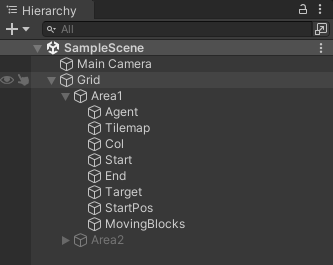
\includegraphics[width=8.8cm]{peliobjektilistaus.png}
\caption{Lista peliobjekteista avoimessa näkymässä. Sisäkkäiset peliobjektit ovat lapsiobjekteja.}
\label{peliobjektikuva}
\end{figure}

\subsection{Komponentit}

Komponentit antavat peliobjekteille ominaisuuksia ja toiminnallisuuksia kuten muodon, värin tai fysiikan. Komponentteja voi olla rajattomasti, mutta peliobjektilla on luonnin jälkeen vähintään Transform-komponentti, joka määrittää peliobjektin sijainnin, suunnan ja skaalan. Transform-komponenttia ei voi poistaa peliobjektilta. Esimerkiksi valmis 3D-objekti pallo (sphere) saa automaattisesti Mesh Filter-, Mesh Renderer- ja Sphere Collider-komponentit. Kaksi ensimmäistä komponenttia keskittyvät pallon graafisiin ominaisuuksiin ja Sphere Collider fyysisiin törmäysominaisuuksiin. Sphere Collider-komponentti asettuu automaattisesti pallon graafisen ulkomuodon kokoiseksi.

Usein komponenteilla on erilaisia arvoja, kuten koko tai väri, joita voi muokata käyttöliittymäelementtien avulla. Komponentit voivat sisältää myös viittauksia muihin peliobjekteihin, tiedostoihin tai assetteihin(käännös?). Esimerkiksi Sprite Renderer -komponenttiin voidaan lisätä viittaus kuvatiedostoon, jolloin Unity renderöi peliobjektin kohdalle lisätyn kuvan. Kuviossa \ref{komponenttikuva} on lista peliobjektin komponenteista ja 

\begin{figure}[h]
\centering
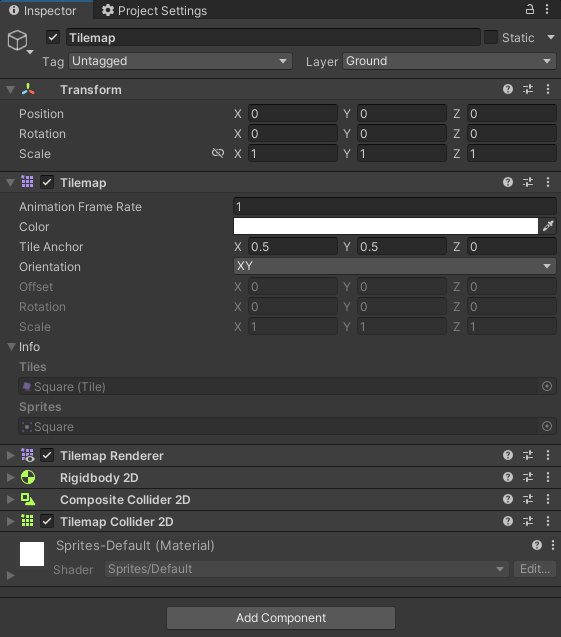
\includegraphics[width=14.8cm]{komponenttilistaus.png}
\caption{Lista peliobjektin komponenteista.}
\label{komponenttikuva}
\end{figure}

\subsection{Skriptit}

Ohjelmoinnin merkitys Unityn käytössä tulee skripteistä. Skriptit ovat ohjelmakooditiedostoja, joita voi lisätä peliobjektiin komponentin tavoin, jos valmiit komponentit eivät riitä toiminnallisuuksiltaan. Skripteissä voi esimerkiksi määritellä ominaisuuksia ja arvoja, joita voi muokata komponenttilistauksessa tai ajon aikana. Unity tukee tällä hetkellä vain C-\# -ohjelmointikieltä, mutta ennen myös Javascriptiin pohjautuvaa UnityScript-ohjelmointikieltä.

Unity tarjoaa skripteihin MonoBehaviour-pohjaluokan, joka mahdollistaa pelinkehityksen tärkeimmät osat eli Start()-aloitusfunktion ja Update()-päivitysfunktion. Start()-funktio ajetaan ennen yhtäkään päivitysfunktiota, joten siinä voidaan määrittää ja alustaa tarvittavat alkuarvot. Update()-funktio ajetaan joka ruudunpäivityskerralla, joten siihen sijoitetaan usein pelilogiikka ja mahdollisesti fyysiset toiminnallisuudet.

Skriptien avulla voidaan tehdä lähes kaikki samat asiat kuin Unity Editorissa. Peliobjekteja voidaan etsiä tagien tai nimien kautta ja niille voidaan lisätä ja poistaa komponentteja ajon aikana. Käyttämättömät peliobjektit voidaan tuhota tai asettaa epäaktiivisiksi jos niitä ei tarvita.

\section{Machine Learning Agents}

Machine Learning Agents on Unitylle kehitetty ilmainen koneoppimispaketti, joka mahdollistaa Unity Editorilla luotujen simulaatioympäristöjen ja Python APIn välisen vuorovaikutuksen. ML-Agents SDK (Software Development Kit) tarjoaa kaikki toiminnallisuudet ja skriptit toimivan koneoppimisympäristön luomiseen. \parencite{juliani2018unity}.

\subsection{ML-Agents SDK}

ML-Agents SDK sisältää kolme ydinosaa: sensorit, agentit ja akatemia. Agentti-komponentti voidaan lisätä suoraan Unityn peliobjektille, jolloin se pystyy keräämään havaintoja, suorittamaan toimintoja ja vastaanottamaan palkkioita. Sensorit mahdollistavat havaintojen keräämisen eri tavoin. Akatemia ylläpitää tietoa simulaation askelmäärästä ja ympäristön parametreista sekä ohjaa agenttien toimintaa.

Agentin käytäntö määritellään Behavior Name -nimikkeen avulla. Eri agenteilla voi olla sama käytäntö, jolloin agentit käyttävät kyseistä käytäntöä päätöksentekoon ja jakavat harjoitteludatan keskenään. Myös useiden erilaisten agenttien toiminta voidaan mahdollistaa erinimisillä käytännöillä.

\subsection{Python API ja PyTorch}

Python APIa käytetään Unityllä tehdyn simulaatioympäristön ja koneoppimissilmukan käsittelyyn. APIn avulla tekijän ei tarvitse itse olla suoraan yhteydessä Pythonin koneoppimiskouluttajaan, vaan API tarjoaa helppokäyttöiset, valmiit menetelmät koneoppimissilmukan luomiseen. Tarkemmin APIsta ja sen toiminnasta voi lukea dokumentaatiosta (tähän linkki sivun alalaitaan tulevasta docsista?).

PyTorch on avoimen lähdekoodin koneoppimiskehys, johon pohjautuen Unity ML-agents -paketin koneoppimiseen liittyvät toteutukset on tehty (Unity ML agents docs). PyTorch sisältää kaikki syvän koneoppimisen perusosat datan kanssa työskentelystä ja koneoppimismallin luomisesta mallin parametrien optimointiin ja oppimismallien tallentamiseen (PyTorch docs).

\chapter{Tutkimuksen empiirinen osuus}

Tässä kappaleessa käsitellään tutkimuksen empiiristä osuutta. Tutkimus toteutettiin empiirisenä vertailevana tutkimuksena. Vertailun kohteena olivat Unityn ML-agentin suorittama reitinhaku ja heuristiseen A*-algoritmiin perustuva reitinhaku. Kappaleessa \ref{sec:tutkimuksenkuvaus} kuvaillaan tutkimusta yleisellä tasolla ja esitellään tutkimuksessa käytetyt työkalut. Kappaleessa \ref{sec:tutkimusasetelma} käydään läpi simulaatioympäristöt ja koneoppimiseen liittyvät konfiguraatiot. Lopuksi kappaleessa \ref{sec:mittaaminen} käsitellään tulosten mittaamista ja käytettyjä suureita.

\section{Tutkimuksen kuvaus}
\label{sec:tutkimuksenkuvaus}

Tutkimuksen simulaatioalustana käytettiin Unityä, koska sen käyttö oli ennestään tuttua ja se soveltuu hyvin erilaisten tilanteiden simuloimiseen. Tutkimusta varten luotiin valmis 2D-projekti, koska tarkoituksena on tutkia kaksiulotteista reitinhakua. Projektiin lisättiin Unity Package Managerin avulla ML-Agents -paketti, jotta tarvittavat toiminnallisuudet saatiin käyttöön koneoppimista varten. Unityllä luotiin yksinkertaisia ruudukkoalueita, jonne sijoitettiin esteruutuja, kävelykelpoisia ruutuja ja maali- ja loppuruutu. Reitinhaun vertailua varten luotiin A*-algoritmi ja opetettiin koneoppimisagentti. Koneoppimisagentti käyttää syvään vahvistettuun oppimiseen perustuvaa SAC-algoritmia.

\section{Tutkimusasetelma / Konfiguraatio}
\label{sec:tutkimusasetelma}

Koneoppimisagentin toiminta riippuu vahvasti sen asetuksista.

- AddObservation()-funktion avulla agentti kerää tietoa omasta tilastaan ympäristössä. Tässä tutkimuksessa agentin täytyy kerätä tietoa sen omasta sijainnista (x ja y), mahdollisesti etäisyydestä maaliin (toimisiko esim. laskea manhattan-etäisyys?) ja maalin sijainnista (x ja y). Suositeltavaa kuitenkin on, että agentti keräisi tietoa vain näkemistään asioista eli tässä tapauksessa vain omasta sijainnistaan. Näiden havaintojen lisäksi käytetään RayPerceptionSensor2D-komponenttia, joka kerää ympäröivästä alueesta tietoa säteiden avulla. Tässä projektissa agentista lähetetään 12 sädettä, jotka yltävät vain yhden ruudun verran eteenpäin. Säteet pystyvät tunnistamaan vastaantulevia objekteja, joita ovat tässä tapauksessa esteet ja maaliruutu. Näiden havaintojen avulla agentti voi tehostaa päätöksentekoaan.

- Actions, toiminnat, yksinkertaisen pelialueen takia käytetään Discrete Actions ja viittä eri vaihtoehtoa (ylös, alas, oikealle, vasemmalle, paikallaan). Jos pelialue olisi monimutkaisempi, voidaan käyttää Continuous Actions (suunta + nopeus).

- Rewards, palkinnot, agentti saa positiivisen palkkion kun saapuu maaliin (+1). Agentti saa negatiivisen palkkion jokaisen toiminnan (action) jälkeen (-0.01). Jos agentti törmäilee seiniin, eli yrittää liikkua suuntaan jossa on este, agentille annetaan negatiivinen palkkio (-0.001). Palkkiot määritellään skriptitiedostossa ja ovat helposti muutettavissa.

- Agentin opettaminen aloitetaan komentoriviltä komennolla ml-agents "BehaviorName"... (myös jotain muuta, ml-agents -komento hyödyntää siis Python APIa). Komentorivi näyttää käyttäjän asettamien opetusaskelten välein mm. agentin keskiarvopalkkion askelten aikana. Tässä tutkimuksessa asetettiin väliksi 10000, tensorboard päivittyy myös 10000 välein ts. piirtää kuvaajan pisteen?

\section{Tulosten mittaaminen}
\label{sec:mittaaminen}

- Reitinhakutehtävästä otetaan talteen aika (sekuntia) ja onnistuiko reitinhaku vai ei (onnistui/epäonnistui).

\chapter{Tulokset ja johtopäätökset}

\chapter{Yhteenveto}

\printbibliography

\chapter{Liitteet}

- Kuvat tai mallinnokset pelialueesta.

- Tensorboardin kuvaajat mm. agentin palkkioiden kehityksestä.

\end{document}
